\documentclass{article}

\title{Transposing tensor files}
\subtitle{Where does file metadata belong?}
\date{2024-11-22}
\modified{2024-11-22}

\keyword{programming}
\keyword{maching-learning}

\begin{document}

\epigraph{
  Here is a problem related to yours and solved before.
  Could you use it?
}{G. Pólya, ``How to Solve It'', second edition, p. 9}

\section*

I recently spent much time working with machine learning serialization formats,
especially \href{https://onnx.ai/}{\textsc{onnx}}.
This file format uses \href{https://protobuf.dev/}{Protocol Buffers} for its binary representation
and inherits the \href{https://protobuf.dev/programming-guides/proto-limits/#total}{two-gigabyte restriction on the file format size}.
Bypassing this restriction requires storing raw tensor bytes
in another file and referencing them from the \textsc{onnx} file.

But what should the tensor file format be?
The \href{https://huggingface.co/docs/safetensors/index}{safetensors} library from Huggingface is popular for representing tensors on disk,
and its data layout is fully compatible with the \textsc{onnx} raw tensor data format.

This article describes the safetensors file structure,
points out its minor design flaws,
and explains how changing the metadata location can address them.

\section{safe-tensors}{The safetensors file format}

A \code{safetensors} file stores a collection of multi-dimensional arrays.
Its first eight bytes indicate the header size as an unsigned 64-bit integer,
follows the header describing each tensor's type and shape,
and then comes the data section containing flat arrays.

\begin{figure}[grayscale-diagram]
  \marginnote{mn-safetensors-structure}{
    The structure of a safetensors file.
    The first eight bytes indicate the header size in bytes.
    The header is a \textsc{json} object describing the tensor metadata.
    The last section contains raw array elements.
  }
  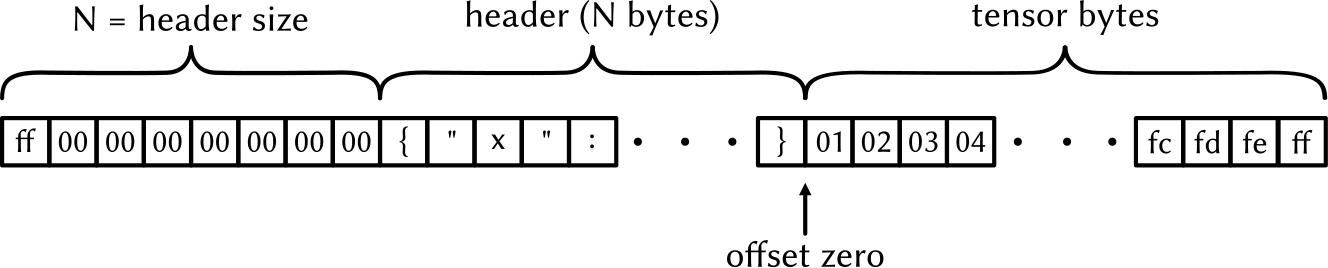
\includegraphics{/images/33-safetensors-structure.svg}
\end{figure}

The header is a \textsc{json} object,
where the key is the tensor name, and the value is an object describing the tensor shape, element type, and offsets from the start of the data section.

\begin{figure}
\marginnote{mn-safetensors-header-example}{
  An example of the safetensors file header.
  The header is a \textsc{json} object mapping tensor names to their metadata: shape, element type, and offsets from the beginning of the data section.
}
\begin{code}[json]
{ "fc.weight": {
    "dtype": "F32",
    "shape": [10, 784],
    "offsets": [0, 31360]
  },
  "fc.bias": {
    "dtype": "F32",
    "shape": [10],
    "offsets": [31360, 31400]
  }
}
\end{code}
\end{figure}

This simple file organization makes it easy to implement and use in most environments.
Unfortunately, it also has a few flaws:
\begin{enumerate}
\item
  Constructing a safetensors file requires two passes over the dataset:
  one pass to gather the tensor metadata and write the header
  and another to append the raw tensor data to the file.
\item
  The tensor data offsets described in the metadata section are relative to the data section, not absolute within a file.
  This design choice makes working with these files more cumbersome:
  We must add the header size (and the size of this size, eight bytes) to tensor offsets before we can read the tensor data.
  The reason for this inconvenience is a chicken-and-egg problem:
  the absolute offsets depend on the header size,
  and the header size depends on the offsets.
  Safetensors designers used relative offsets in the header to break this cycle.
\item
  The work required to add a new tensor or change the header is proportional to the entire file size,
  not the change size.
\end{enumerate}

\section{tensor-safes}{Tensor safes}

I like to imagine a tensor file as a safe with gold ingots (tensors) inside.
The metadata section is a slip of paper describing each ingot's weight, purity, and location in the safe.
The safetensors layout requires us to fill out the paper first,
place it at the back of the safe,
and assemble the ingots as described.

Luckily, there is an easier way.
Put the ingots first, jotting down the size and location on the paper as you go.
Once all the gold is in the safe, put the paper in front of it and seal it.
In the world of binary files, this idea corresponds to placing the metadata block at the end of the file\sidenote{sn-leveldb}{
  I learned this trick from the \href{https://github.com/google/leveldb/blob/main/doc/table_format.md}{LevelDB table format}.
}.
Let's call this derived format \emph{tensorsafe}.

The format makes two minor adjustments to the \code{safetensors} structure:
\begin{enumerate}
\item The metadata block lives at the end of the file, followed by the metadata size\sidenote{sn-metadata-size-u32}{
  I limited the metadata section size to four bytes on the figure,
  enough to store more than 10,000,000 tensors in a single file, assuming a single entry is under 400 bytes.
}.
\item The file starts with a fixed-size header containing \href{https://en.wikipedia.org/wiki/Magic_number_(programming)#In_files}{magic bytes} and the version.
  All self-respecting file formats need versioning.
\end{enumerate}
\newline

\begin{figure}[grayscale-diagram]
  \marginnote{mn-tensorsafe-structure}{
    The structure of a tensorsafe file.
    The header has a fixed size and includes magic bytes and the version.
    The variable-size metadata block moved to the end of the file.
  }
  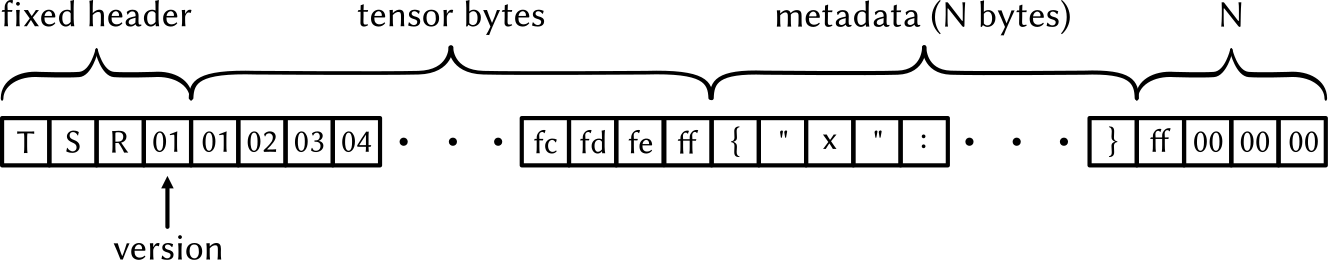
\includegraphics{/images/33-tensorsafe-structure.svg}
\end{figure}

These changes address all my issues with \code{safetensors}:
\begin{enumerate}
\item The encoder needs only one pass over the data.
  It can accumulate the metadata while writing tensors to the file and add the metadata section at the end.
\item
  The metadata section becomes self-contained and can use absolute offsets for tensor boundaries.
  The reader doesn't need to massage the offsets anymore.
\item
  We don't have to move the data to append new tensors:
  We can write over the old metadata section and append the new one.
\end{enumerate}

Are there any new downsides to the \code{tensorsafe} approach?
None that I can think of.

\section{alternative-designs}{Alternative designs}

Dumping the entire metadata section at the beginning or the end of a file are not the only options available.
This section explores other popular approaches for metadata encoding,
such as spreading it across the file or making it float freely.

\subsection{chunked-metadata}{Chunked metadata}

We can represent a collection of items by packaging each item's metadata and data into a distinct chunk.
For example,
\href{https://en.wikipedia.org/wiki/PNG#File_format}{\textsc{png}} encodes various aspects of the image as separate chunks,
and the \href{https://webassembly.github.io/spec/core/binary/index.html}{WebAssembly binary format} represents a module as a collection of sections (types, imports, memory, etc.).

When we apply this approach to tensor encoding,
we interleave tensor attributes with the tensor data.

\begin{figure}[grayscale-diagram]
\marginnote{mn-chunked-metadata}{
  The chunked metadata approach: the tensor file contains a self-contained section for each tensor.
}
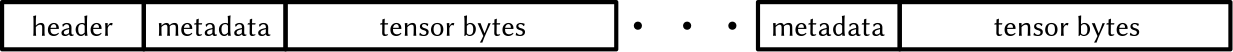
\includegraphics{/images/33-chunked-metadata.svg}
\end{figure}

This approach also addresses the original design issues:
\begin{itemize}
\item The encoder no longer needs to accumulate metadata;
  producing a file requires a single straightforward loop over the tensors.
\item The metadata section doesn't need to contain tensor offsets:
  The decoder can compute them by scanning the file.
\item We can append new tensors to the file without touching existing items.
\end{itemize}

Unfortunately, this design also has a severe disadvantage:
The decoder has to scan the entire file even if the caller is interested in accessing only a specific tensor.
Furthermore, metadata decoding becomes slower because it involves many file seeks.

\subsection{floating-metadata}{Floating metadata}

We explored options where metadata occupies the file's beginning and end
and is spread thinly across it.
Are there any more options?
There are!
The metadata block can float freely within the file\sidenote{sn-floating-wad}{
I first encountered this idea when dealing with \href{https://doomwiki.org/wiki/WAD}{\textsc{wad}} files.
I later learned that \href{https://en.wikipedia.org/wiki/PDF#File_format}{\textsc{pdf}} uses a similar trick for its cross-reference tables.
}.

With this design, a fixed-size file header contains an offset of the metadata block location.
The encoder writes a default header at first,
encodes the entire dataset,
appends the metadata block,
and finally goes back to the header to update the metadata offset.

\begin{figure}[grayscale-diagram]
\marginnote{mn-floating-metadata}{
  The floating metadata approach: a fixed-size header contains the metadata offset.
}
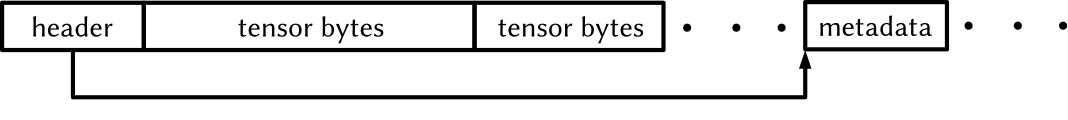
\includegraphics{/images/33-floating-metadata.svg}
\end{figure}

This design has all the benefits of the \href{#tensor-safes}{tensorsafe} format,
and the extra level of indirection adds another feature: \emph{atomic in-place updates}.
You can add, remove, or edit tensors using the following procedure:
\begin{enumerate}
\item Append the new data and a new metadata section to the file.
\item \href{https://www.man7.org/linux/man-pages/man2/fsync.2.html}{Sync} the changes to disk.
\item Update the header to point to the new metadata entry.
\end{enumerate}

This approach guarantees that the file will stay consistent
even if the writing process crashes before completing the update,
but it can lead to extra space usage.
The writer can detect and reuse that space in subsequent updates.

Given modern advances in hardware and file systems,
atomic updates might not be worth the extra complexity.

\section{conclusion}{Conclusion}

This article covered a few alternative designs for the \code{safetensors} file format
and argued that moving the metadata section at the end of the file would make the format easier to use.
The following table summarizes the design space.

\begin{figure}[fullwidth]
\begin{tabular}{r c c c c}
& safetensors & tensorsafe & chunked & floating \\
\hrule
Zero-copy decoding & \dingbat{heavy-check} & \dingbat{heavy-check} & \dingbat{heavy-check} & \dingbat{heavy-check} \\
Fast metadata decoding & \dingbat{heavy-check} & \dingbat{heavy-check} & \dingbat{heavy-ballot-x} & \dingbat{heavy-check} \\
Data passes required for encoding & 2 & 1 & 1 & 1 \\
Absolute file offsets in metadata & \dingbat{heavy-ballot-x} & \dingbat{heavy-check} & n/a & \dingbat{heavy-check} \\
Atomic in-place updates & \dingbat{heavy-ballot-x} & \dingbat{heavy-ballot-x} & \dingbat{heavy-ballot-x} & \dingbat{heavy-check} \\
\end{tabular}
\end{figure}

\section{checklist}{Appendix: binary format checklist}

\begin{checklist}
\item I can explain why I need to design a new binary format.
\item I studied design choices that similar formats made.
\item The file metadata has a version number.
\item I requested a design review from the community.
\item I wrote a detailed specification of my format.
\end{checklist}

\end{document}
